Ye olde superconductors.

\begin{parts}
	\part Standard sketches.
	\begin{subparts}
		\subpart Heed that we have a \underline{type II} SC here $\rightarrow$ vortex state!
		\begin{figure}[H]
			\centering
			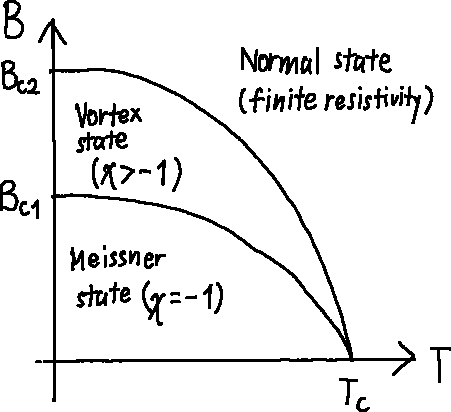
\includegraphics[width=.45\linewidth]{q5-phase}
		\end{figure}
		
		\subpart See Q5 2018 for reference.
		\begin{figure}[H]
			\centering
			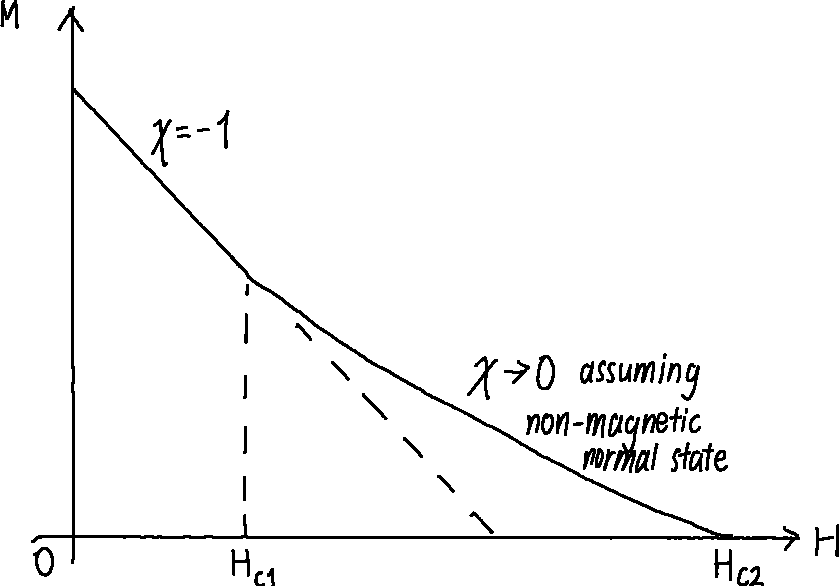
\includegraphics[width=.6\linewidth]{q5-magnetisation}
		\end{figure}
	\end{subparts}
	
	\part A rather strange part.
	I'd say that it tests more on Ampere's Law\footnote{As an anecdote, the author bombed this part by creating a new universe in which Ampere's Law took the form of $\int\mathbf{B}\cdot\inftsml{\mathbf{A}}$\dots} than SC!
	\begin{subparts}
		\subpart By Silsbee's Rule (fancy name for Ampere's Law under critical conditions), we have:
		\begin{equation}
			B_\textnormal{c} \cdot 2\pi r = \mu_0 I_\textnormal{c}
			\label{eqn:q5-silsbee-rule}
		\end{equation}
		where $B_\textnormal{c}$ is the critical/upper-critical $B$ field for type I/II SC, $I_\textnormal{c}$ is the critical current.
		
		Plugging in the dimensions of the Ta and Nb wires given in the question then gives:
		\begin{gather*}
			I_\textnormal{c}^\textnormal{Ta} = \frac{(\SI{0.09}{\tesla})2\pi(\SI{0.1}{\milli\metre})}{\mu_0} = \SI{45}{\ampere} \\
			\Rightarrow J_\textnormal{c}^\textnormal{Ta} = \frac{I_\textnormal{c}^\textnormal{Ta}}{\pi (\SI{0.1}{\milli\metre})^2} = \SI{1.43e9}{\ampere\per\metre\squared} \\
			\\
			I_\textnormal{c}^\textnormal{Nb} = \frac{(\SI{0.19}{\tesla})2\pi(\SI{0.025}{\milli\metre})}{\mu_0} = \SI{23.75}{\ampere} \\
			\Rightarrow J_\textnormal{c}^\textnormal{Ta} = \frac{I_\textnormal{c}^\textnormal{Nb}}{\pi (\SI{0.025}{\milli\metre})^2} = \SI{1.21e10}{\ampere\per\metre\squared}
		\end{gather*}
		
		\subpart The temperature dependence is already given so sketch it!
		
		\begin{figure}[H]
			\centering
			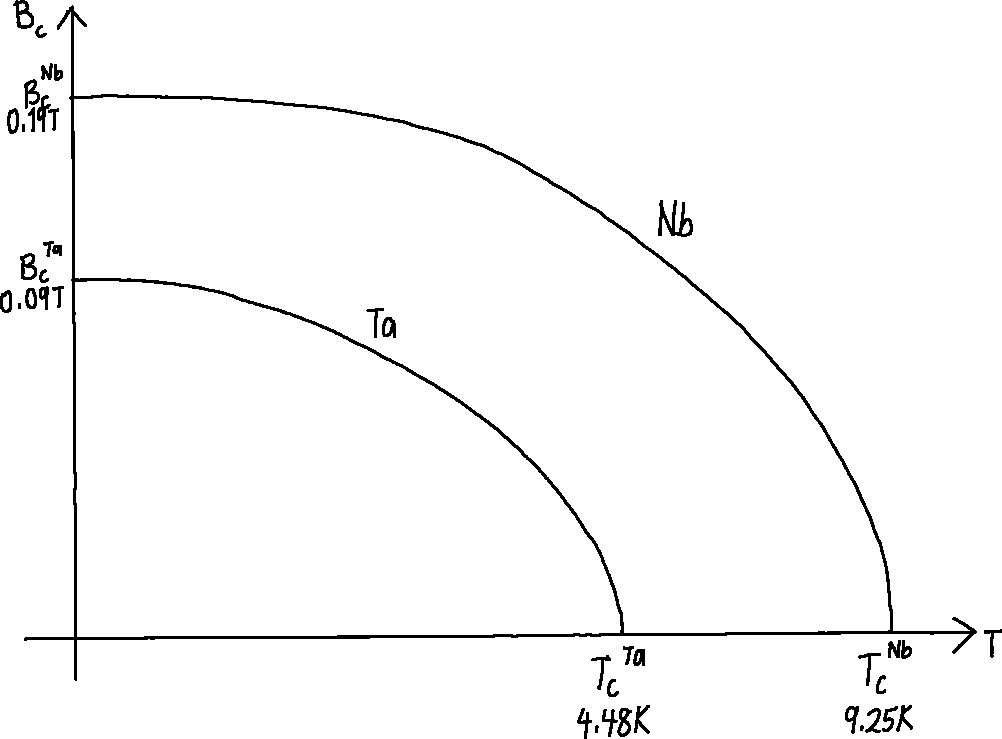
\includegraphics[width=.6\linewidth]{q5-temp-dependence}
		\end{figure}
		
		Note that Nb is superconducting in larger range of $B$ and $T$.
		
		\subpart At $T_1$ we have the critical $B$ field as:
		\begin{equation}
			B_\textnormal{c}(T_1) = B_\textnormal{c}\sbracket{1 - \rbracket{\frac{T_1}{T_\textnormal{c}}}^2}
		\end{equation}
		
		Then by Silsbee's Rule we have the critical current at $T_1$:
		\begin{align*}
			I_\textnormal{c}^\textnormal{Ta}(T_1) &= \frac{B_\textnormal{c}(T_1) \cdot 2\pi r_1}{\mu_0} \\
			&= I_\textnormal{c}^\textnormal{Ta} \sbracket{1-\rbracket{\frac{T_1}{T_\textnormal{c}}}^2} \\
			&= \rbracket{\SI{45}{\ampere}} \sbracket{1-\rbracket{\frac{\SI{4.15}{\kelvin}}{\SI{4.48}{\kelvin}}}^2} \\
			&= \SI{6.39}{\ampere}
		\end{align*}
		
		\subpart Nothing to do with SC since we are only at the surface with no screening!
		
		\begin{figure}[H]
			\centering
			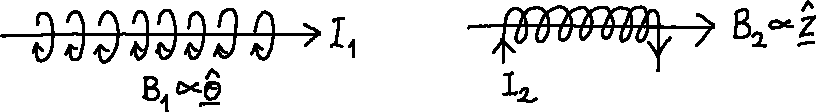
\includegraphics[width=.8\linewidth]{q5-b-field}
		\end{figure}
		
		From the sketch we see that the $B$ field contributions from each wire are perpendicular to each other ($\hat{\bm{\theta}}$ and $\hat{\mathbf{z}}$ in cylindrical coordinates), hence the magnitude of the net $B$ field would be:
		\begin{equation}
			B = \sqrt{B_1^2 + B_2^2}
			\label{eqn:q5-net-b-field}
		\end{equation}
		where $B_{1/2}$ is the $B$ field due to $I_{1/2}$.
		
		By Ampere's Law we then have:
		\begin{gather}
			B_1 = \frac{\mu_0 I_1}{2\pi r_1}
			\label{eqn:q5-b1} \\
			B_2 = \mu_0 \diagfrac{N}{L} I_2
			\label{eqn:q5-b2}
		\end{gather}
		
		So $\alpha = \rbracket{\dfrac{\mu_0}{2\pi r_1}}^2$, $\beta = \rbracket{\dfrac{\mu_0 N}{L}}^2$.
		
		\subpart Equating $B$ with $B_\textnormal{c}^\textnormal{Ta}(T_1)$ and therefore \eqref{eqn:q5-net-b-field} becomes:
		\begin{gather*}
			B_\textnormal{c}^\textnormal{Ta}(T_1) = \sqrt{\alpha I_1^2 + \beta I_2^2} \\
			\Rightarrow \beta = \frac{1}{I_2^2} \sbracket{\rbracket{ B_\textnormal{c}^\textnormal{Ta}(T_1) }^2 - \alpha I_1^2} = \rbracket{\mu_0 n_\textnormal{c}}^2 \\
			\Rightarrow n_\textnormal{c} = \frac{1}{\mu_0 I_2} \sqrt{\rbracket{ B_\textnormal{c}^\textnormal{Ta}(T_1) }^2 - \alpha I_1^2} = \SI{1.02e5}{\per\metre} = \SI{102}{\per\milli\metre}
		\end{gather*}
		where $n_\textnormal{c} = (\diagfrac{N}{L})_\textnormal{c}$ is the critical number of turns per unit length beyond which the Ta wire becomes resistive.
	\end{subparts}
	
	\part Simple question on BCS theory.
	\begin{subparts}
		\subpart Recall from BCS theory that $\lambda = g(E_\textnormal{F}) \abs{g_\textnormal{eff}}^2$ is the phonon-electron coupling parameter -- it encodes the interaction between phonon and electron near the Fermi surface and has been shown to be attractive by Cooper.
		
		$\hbar\omega_\textnormal{D}$ is the energy at Debye frequency -- in Cooper's theory this is the upper energy limit for which the electron-phonon interaction remains attractive.
		
		Both parameters suggest that an electron pair may form under low temperature, this is called the Cooper pair.
		
		\newpage
		\subpart Usual sketch from lecture notes, note that the Cooper pair I have drawn corresponds to the ground state where there is no centre-of-mass motion.
		
		\begin{figure}[H]
			\centering
			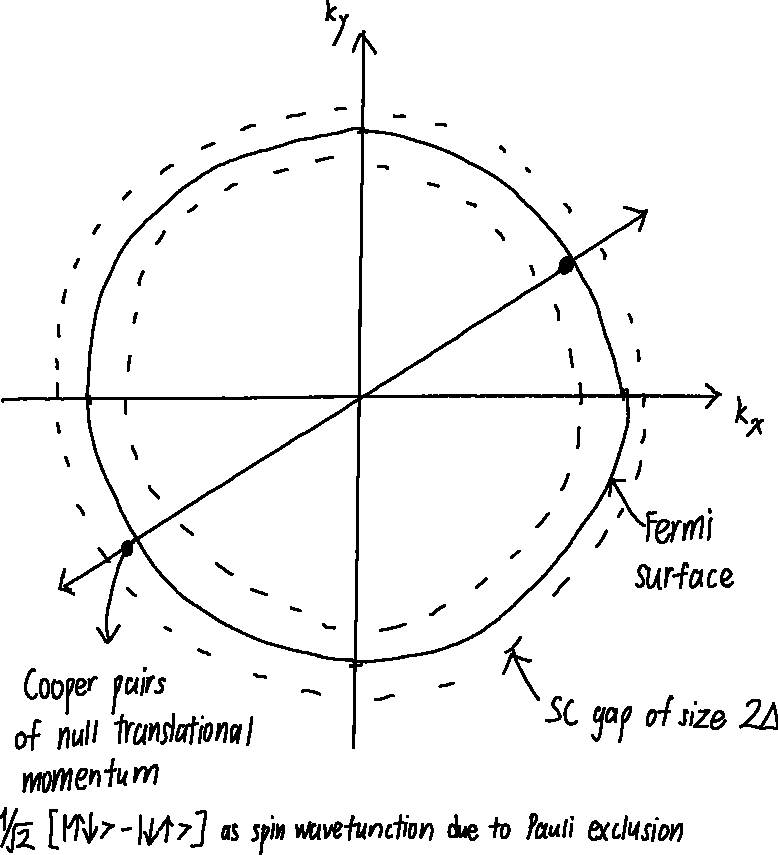
\includegraphics[width=.8\linewidth]{q5-cooper-pair}
		\end{figure}
		
		\newpage
		\subpart From the given gap equation,
		\begin{equation}
			\lambda \int_{0}^{\hbar\omega_\textnormal{D}} \inftsml{\epsilon} \frac{1}{\sqrt{\epsilon^2 + \Delta^2}} = 1
			\label{eqn:q5-gap-equation}
		\end{equation}
		
		Taking the limit of $\Delta \ll \hbar\omega_\textnormal{D} \Rightarrow \hbar\omega_\textnormal{D} / \Delta \gg 1$ yields:
		\begin{gather}
			\lambda \int_{0}^{\hbar\omega_\textnormal{D}} \frac{\inftsml{\epsilon} / \Delta}{\sqrt{1 + (\epsilon/\Delta)^2}} = 1 \notag \\
			\Rightarrow \lambda \int_{0}^{\hbar\omega_\textnormal{D} / \Delta} \frac{\inftsml{x}}{\sqrt{1+x^2}} = 1 \textnormal{\hspace{1em}where $x=\epsilon/\Delta$} \notag \\
			\sinh^{-1} \rbracket{\frac{\hbar\omega_\textnormal{D}}{\Delta}} - \sinh^{-1} 0 = \frac{1}{\lambda} \notag \\
			\Rightarrow \ln \rbracket{\sqrt{\rbracket{\frac{\hbar\omega_\textnormal{D}}{\Delta}}^2 + 1} + \rbracket{\frac{\hbar\omega_\textnormal{D}}{\Delta}}} - 0 = \frac{1}{\lambda} \notag \\
			\Rightarrow \ln \sbracket{ 2 \rbracket{\frac{\hbar\omega_\textnormal{D}}{\Delta}} } = \frac{1}{\lambda} \textnormal{\hspace{1em}since $\hbar\omega_\textnormal{D} / \Delta \gg 1$} \notag \\
			\Delta = 2\hbar\omega_\textnormal{D} e^{-1/\lambda}
			\label{eqn:q5-energy-gap}
		\end{gather}
		
		\subpart Substituting $\hbar\omega_\textnormal{D} = k_\textnormal{B}T_\textnormal{D}$, $T_\textnormal{D} \approx \SI{276}{\kelvin}$ and $\lambda \approx 0.1$ into \eqref{eqn:q5-energy-gap} gives:
		\begin{align*}
			\Delta &= 2k_\textnormal{B}T_\textnormal{D} e^{-1/\lambda} \\
			&= \SI{3.46e-25}{\joule} \\
			&= \SI{2.16e-6}{\electronvolt}
		\end{align*}
		
		\textit{Aside: It doesn't fit the measured value of $2\Delta = \SI{3.8}{\milli\electronvolt}$? This paper\footnote{Superconductivity in Nb: Impact of Temperature, Dimensionality and Cooper-Pairing: \url{https://doi.org/10.3390/nano14030254}} suggests that $\lambda \approx \SI{1.1}{\electronvolt}$ for the magnitude to match.}
	\end{subparts}
\end{parts}